\begin{frame}[allowframebreaks]{Super-Resolution}

Autoencoders can be used to reconstruct high-resolution images from their low-resolution counterparts.

\begin{itemize}
    \item Input: Low-resolution image.
    \item Output: High-resolution image.
    \item Often implemented with convolutional layers for spatial pattern learning.
\end{itemize}
\textbf{Use Case}: Enhancing medical images, satellite images, or upscaling low-resolution photos.

\framebreak

\begin{figure}
    \centering
    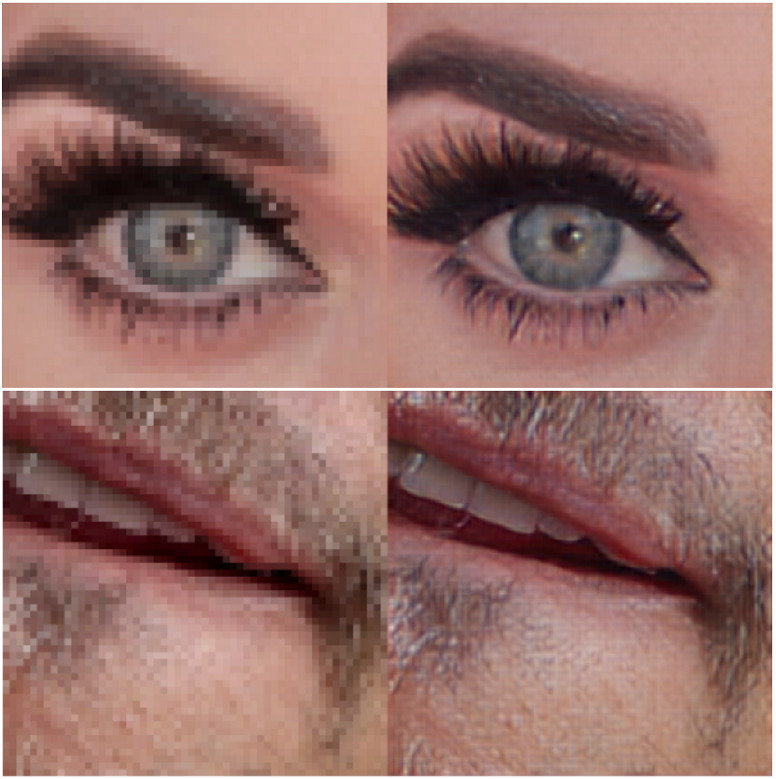
\includegraphics[height=0.8\textheight, width=\textwidth, keepaspectratio]{./images/autoencoders/image_enhancement.png}
    \caption*{Image super-resolution using Autoencoders}
\end{figure}

\end{frame}